\documentclass{article}
\usepackage[utf8]{inputenc}
\usepackage{tikz}
\usepackage{amsmath}
\usepackage{enumitem}
\usepackage[a4paper, margin=2cm]{geometry}

\begin{document}
	
	\begin{center}
		\begin{minipage}[t]{0.48\textwidth}
			\centering
			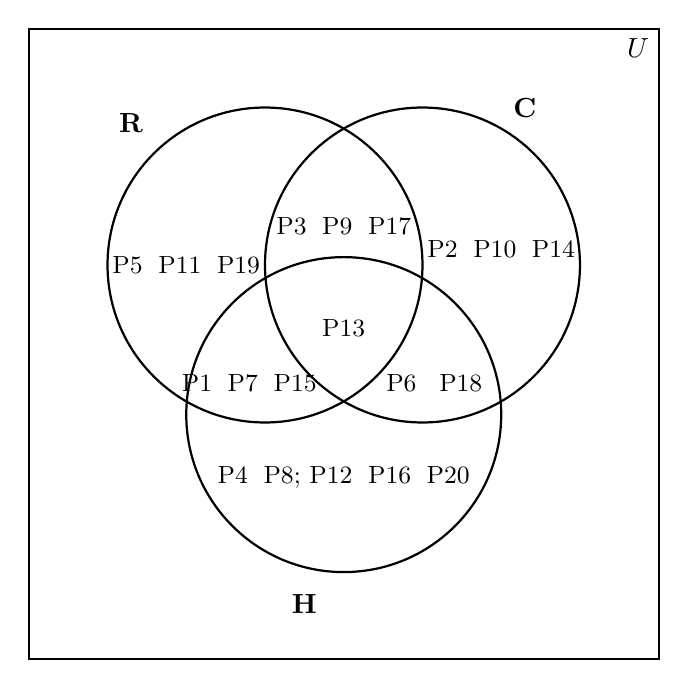
\begin{tikzpicture}
				% Rectángulo del universo
				\draw[thick] (-3,-3) rectangle (5,5);
				\node[anchor=north east] at (5,5) {\(U\)};
				
				% Círculos de los conjuntos
				\draw[thick] (0,2) circle (2cm);      % H
				\draw[thick] (2,2) circle (2cm);      % D
				\draw[thick] (1,0.1) circle (2cm);    % C
				
				% Etiquetas de los conjuntos
				\node at (-1.7, 3.8) {\textbf{R}};
				\node at (3.3, 4) {\textbf{C}};
				\node at (0.5,-2.3) {\textbf{H}};
				
				% Elementos en cada región
				\node at (-1, 2) {\small P5\; P11\; P19};               % Solo H
				\node at (3, 2.2) {\small P2\; P10\; P14};                % Solo D
				\node at (1,-0.7) {\small P4\; P8; P12\; P16\; P20};              % Solo C
				\node at (1,2.5) {\small P3\; P9\; P17};                    % H ∩ D
				\node at (-0.2,0.5) {\small P1\; P7\; P15 };                     % H ∩ C
				\node at (2.15,0.5) {\small P6\; \;P18};                         % D ∩ C
				\node at (1,1.2) {\small P13};                      % H ∩ D ∩ C
				%\node at (3.5,-2) {\small 11\; 18};                     % Fuera de los conjuntos
			\end{tikzpicture}
		\end{minipage}
		\hfill
		\begin{minipage}[t]{0.48\textwidth}
			\raggedright
			\begin{itemize}[leftmargin=*]
				\item[] \( H \cap D \cap C = \{5, 6\} \)
				\item[] \( H \cap D = \{3, 4, 5, 6\} \)
				\item[] \( H \cap C = \{5, 6, 7, 8\} \)
				\item[] \( D \cap C = \{5, 6, 12\} \)
				\item[] \( \text{Solo } H = \{1, 2, 9, 10\} \)
				\item[] \( \text{Solo } D = \{13, 14, 15\} \)
				\item[] \( \text{Solo } C = \{16, 17, 19, 20\} \)
				\item[] \( H \cup D \cup C = \{1, 2, 3, 4, 5, 6, 7, 8, 9, 10, 12, 13, 14, 15, 16, 17, 19, 20\} \)
				\item[] \( (H \cup D \cup C)^c = \{11, 18\} \)
			\end{itemize}
		\end{minipage}
	\end{center}
	
\end{document}
